\documentclass[a0,portrait]{a0poster}

\usepackage{multicol} % This is so we can have multiple columns of text side-by-side
\columnsep=100pt % This is the amount of white space between the columns in the poster
\columnseprule=2pt % This is the thickness of the black line between the columns in the poster
\usepackage{times}
\usepackage[font=small,labelfont=bf]{caption}
\usepackage{wrapfig}
\usepackage{amsmath}
\usepackage{amsfonts}
\usepackage{amsthm}
\usepackage{bibentry}
\usepackage{graphicx}
\usepackage{bm}
\usepackage{booktabs}
\usepackage{tikz}
\usepackage{xcolor}
\usepackage{multirow}
\usepackage[normalem]{ulem}
\usepackage{pifont}
\usepackage{array}
\usepackage{sectsty}
% \allsectionsfont{\centering}
\graphicspath{{figures/}, {../images/}, {../auto_fig/}}

\definecolor{l10_color1}{HTML}{3232FF}
\definecolor{coloranswer}{HTML}{0596FF}
\definecolor{lightblue}{HTML}{3CC7EA}
\definecolor{boxcolor}{HTML}{EEEEEE}
\definecolor{periwinkle}{rgb}{0.8, 0.8, 1.0}
\definecolor{colorsquad}{rgb}{0,1,0}
\definecolor{colorsnli}{rgb}{1,0,0}
\definecolor{colorvqa}{rgb}{1,1,0}

\newcommand\BibTeX{B{\sc ib}\TeX}
\newcommand{\abr}[1]{\textsc{#1} }
\newcommand{\squad}{\textsc{SQuAD}}
\newcommand{\snli}{\textsc{SNLI}}
\newcommand{\vqa}{\textsc{VQA}}
\newcommand{\nlp}{\textsc{nlp}}
\newcommand{\mb}[1]{\boldsymbol{\mathbf{#1}}}
\newcommand{\loo}{leave-one-out}
\newcommand{\g}{\, | \,}

\begin{document}

%----------------------------------------------------------------------------------------
%	POSTER HEADER 
%----------------------------------------------------------------------------------------

% The header is divided into two boxes:
% The first is 75% wide and houses the title, subtitle, names, university/organization and contact information
% The second is 25% wide and houses a logo for your university/organization or a photo of you
% The widths of these boxes can be easily edited to accommodate your content as you see fit

\begin{minipage}[b]{1\linewidth}
\centering
\veryHuge \color{blue} \textbf{Pathologies of Neural Models Make Interpretations
Difficult} \\[0.4cm]
\color{black}\LARGE
Shi Feng$^1$ Eric Wallace$^1$ Alvin Grissom~II$^2$ Mohit Iyyer$^{3,4}$ Pedro Rodriguez$^1$ Jordan Boyd-Graber$^1$\\[0.4cm]
\Large
\textit{$^1$University of Maryland $^2$Ursinus College $^3$UMass Amherst $^4$Allen Institute for Artificial Intelligence}\\
\end{minipage}

\vspace{0.6cm}

\begin{multicols}{2}

\large

\section*{Abstract}
One way to interpret a neural text classifier is to highlight the most important
words in the input. Existing methods of word importance estimate reply largely
on model confidence---either directly by removing each word from the input, or
indirectly with input gradient. To understand the limitations of
confidence-based interpretation, we use input reduction, which iteratively
removes the least important word. Input reduction produces nonsensical examples
that trigger the same model prediction with high confidence. We explain this
type of pathological behavior from the perspective of uncertainty estimate and
adversarial examples. To mitigate the model deficiencies, we take the reduced
examples and impose an entropy regularization. Fine-tuned models become more
interpretable under input reduction without accuracy loss on regular examples.
\vspace{0.6cm}

\section*{Pathological Examples}
Neural models are known to have issues...

\vspace{0.6cm}
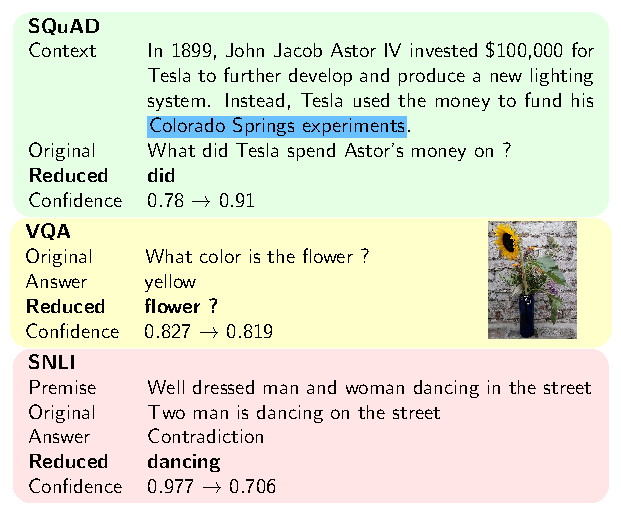
\includegraphics[width=\linewidth]{21}
\vspace{0.6cm}

\section*{Input Reduction}
How do we generate those examples?

\begin{center}\vspace{0.6cm}
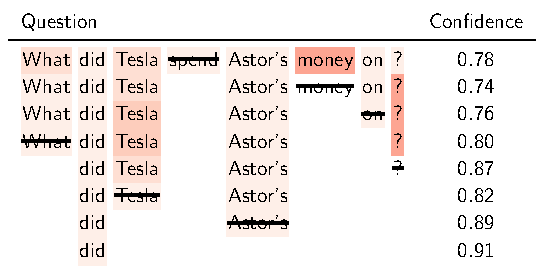
\includegraphics[width=0.9\linewidth]{15}
\end{center}\vspace{0.6cm}


\section*{Leave-One-Out}
Input reduction is not stupid...

\begin{center}\vspace{0.6cm}
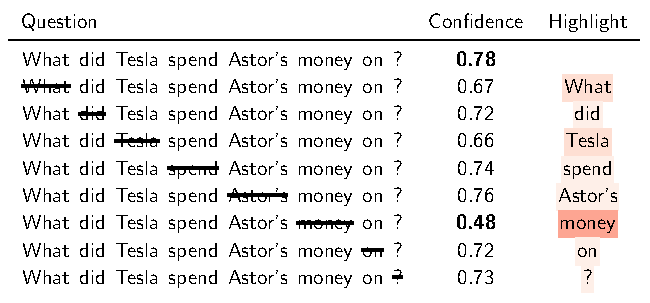
\includegraphics[width=0.9\linewidth]{9}
\end{center}\vspace{0.6cm}

\vfill\null
\columnbreak

\section*{On the Dataset Scale}
This happens on the dataset scale...

\begin{center}\vspace{0.6cm}
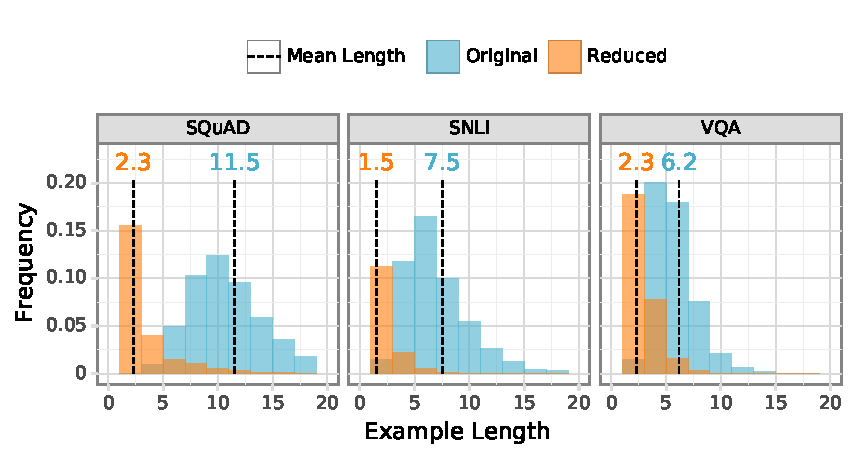
\includegraphics[width=0.9\linewidth]{length_histogram}
\end{center}

\begin{center}
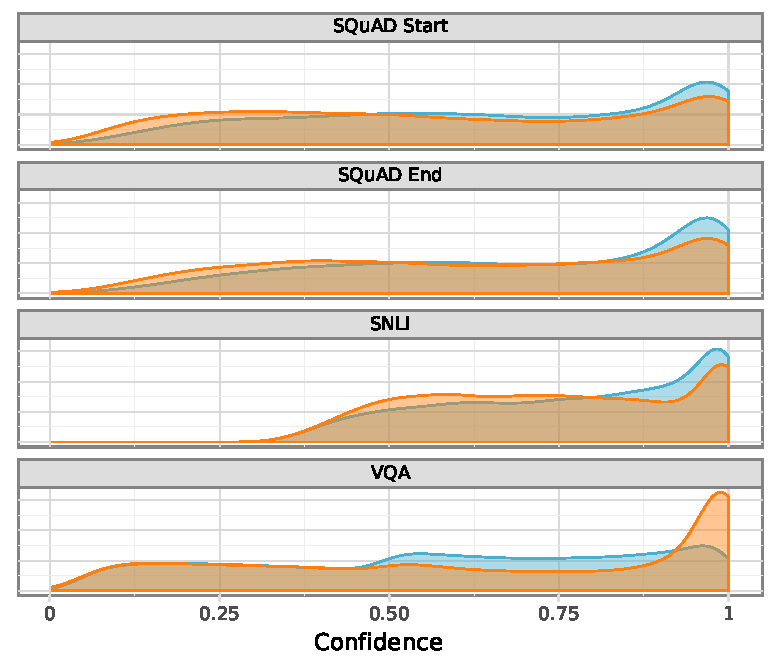
\includegraphics[width=0.6\linewidth]{confidence}
\end{center}\vspace{0.6cm}


\section*{Human Are Confused}
The reduced examples are indeed nonsensical...

\begin{center}\vspace{0.6cm}
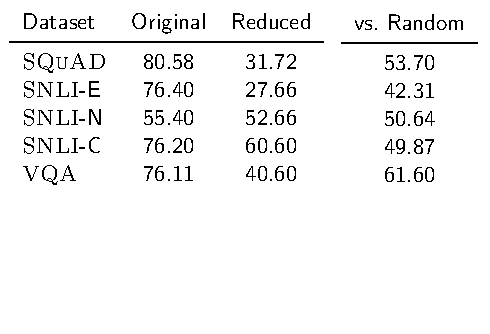
\includegraphics[width=0.8\linewidth]{29}
\end{center}\vspace{0.6cm}


\section*{Heatmap Shifts}
Importance measured individually ignores high-order correlation between words...

\begin{center}\vspace{0.6cm}
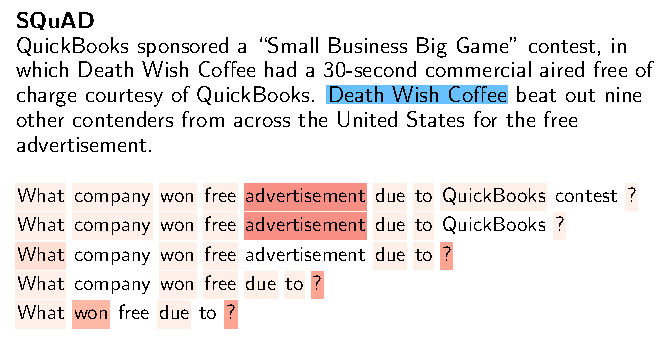
\includegraphics[width=0.9\linewidth]{42}
\end{center}\vspace{0.6cm}


\section*{Mitigation}
There is still hope...

\begin{center}
\begin{equation}
\sum_{(\mb{x}, y)}\log(f(y \g \mb{x})) \
+ \lambda\sum_{\tilde{\mb{x}}\in \tilde{\mathcal{X}}}
\mathbb{H}\left(f(y \g \tilde{\mb{x}})\right) \nonumber
\end{equation}
\end{center}

% \vspace{0.6cm}
% 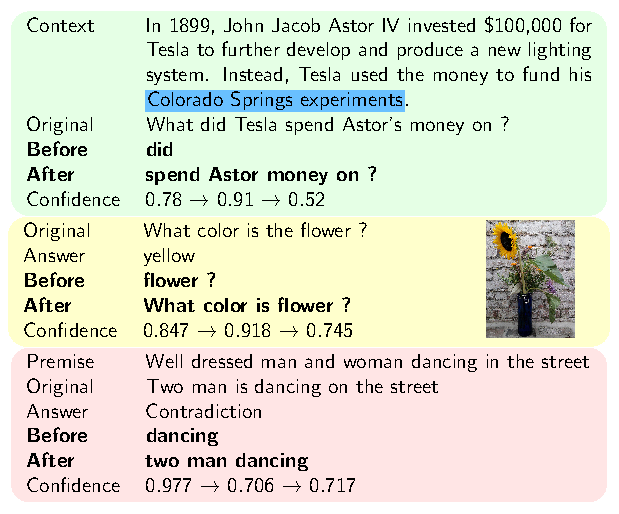
\includegraphics[width=0.9\linewidth]{48}
% \vspace{0.6cm}
% 
% \vspace{0.6cm}
% 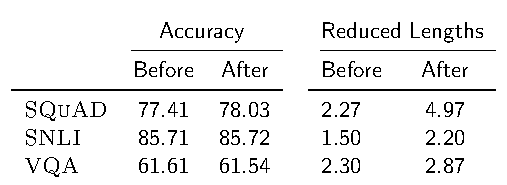
\includegraphics[width=0.9\linewidth]{50}
% \vspace{0.6cm}
% 
% \vspace{0.6cm}
% 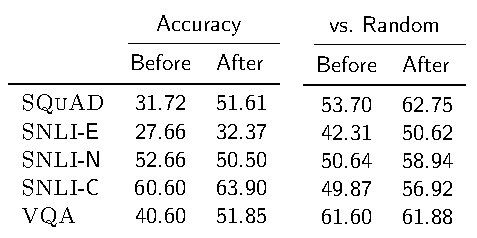
\includegraphics[width=0.9\linewidth]{57}
% \vspace{0.6cm}


\section*{Conclusions}
\begin{itemize}
\item Confidence of a neural model trained with MLE is not reliable for
interpretation
\item Existing interpretation methods ignore high-order correlation between
words
\end{itemize}

% \section*{Referencias}
% \bibliographystyle{plain} % Plain referencing style
% \bibliography{journal-abbrv,fs}

\end{multicols}
\end{document}
